\documentclass[11pt,xcolor={dvipsnames},hyperref={pdftex,pdfpagemode=UseNone,hidelinks,pdfdisplaydoctitle=true},usepdftitle=false]{beamer}
\usepackage{presentation}

% Enter presentation title to populate PDF metadata:
\hypersetup{pdftitle={Minimalist LaTeX Template for Academic Presentations}}

% Enter path to PDF file with figures:
\newcommand{\pdf}{figures.pdf}

\begin{document}

% Enter title:
\title{Risk Models From Tree-Structured MRFs Following Multivariate Poisson Distributions}


\information
%
% Enter URL to research paper (can be commented out):
% [https://arxiv.org/pdf/2412.00607]
%
% Enter authors:
{
\Large Alexandre Dubeau\\
% \vspace{-1cm}
\smallskip \large Joint work with H. Cossette, B. Côté, and E. Marceau\\
\normalsize École d'actuariat, Université Laval}
%
% Enter location and date (can be commented out):
{Statistical Society of Canada Conference-- May 26 2025}

\frame{\titlepage}

\section{Introduction}
\begin{frame}{Two Major Insurance Systems}
\begin{minipage}[t]{0.45\textwidth}
{\large Traditional Insurance}:
\begin{itemize}
    \item Centralized risk-sharing mechanism;
    \item Insurer = intermediary;
    \item Standardized contracts $\Rightarrow$ portfolio expansion.
    % \item  Focus on predictability and accessibility
\end{itemize}
\end{minipage}
\hfill
\begin{minipage}[t]{0.45\textwidth}
{\large Decentralized Insurance}\\
\citep{feng2024unified}:
\begin{itemize}
    \item Removal of a central intermediary;
    \item Reform of mutualization principles;
    \item Use of modern technologies.
\end{itemize}
\end{minipage}
\pause

\vspace{5pt}

{\large Common point: }
\begin{itemize}
    \item Based on risk pooling;
    \item One of the objectives: \\
    $\downarrow$ individual contributions through \al{risk sharing}.
\end{itemize}
\end{frame}



\begin{frame}[label=toc]{Overview}
    \setlength{\leftskip}{5cm}%
    \tableofcontents[subsectionstyle=hide]
\end{frame}

\section{Individual Risk Models and Risk Sharing}
\begin{frame}{Individual Risk Model - Classical Framework}
Definition: 
\begin{itemize}
    \item Portfolio of $n$ participants $\boldsymbol{X} = (X_i)_{i=1}^{n}$.
    \item Each has a non-negative monetary loss $X_i, i \in [n]$.
    \item $\mu_i = \mathbb{E}[X_i] < \infty$, $\sigma_i^2 = \mathrm{Var}(X_i) < \infty$.
    \item Aggregate portfolio loss $S_n$:  
    \begin{equation*}
    S_n = X_1 + X_2 + \cdots + X_n.
    \end{equation*}
\end{itemize}
\vfill

\pause

Assumptions about the random variables $X_i$: 
\begin{itemize}
    \item identically distributed (homogeneous portfolio);
    \item independent.
\end{itemize}
\end{frame}


\begin{frame}{Risk Sharing: Definition and Optimal Rule}

    \begin{itemize}
        \item \al{Fair risk sharing rule:} a function $h: \boldsymbol{X} \mapsto (h_{i,n}(S_n))_{i \in [n]}$ that allocates the total cost $S_n = \sum_{i=1}^n X_i$ among $n$ participants such that:
        \begin{equation*}
        \sum_{i=1}^n h_{i,n}(S_n) = S_n
        \quad \text{and} \quad
        \mathbb{E}[h_{i,n}(S_n)] = \mathbb{E}[X_i] \quad \text{(fairness)}.
        \end{equation*}
        \pause
        \item \al{Optimal rule:} the conditional expectation
        \begin{equation*}
        h_{i,n}^{\star}(S_n) = \mathbb{E}[X_i \mid S_n]
        \end{equation*}
        minimizes the mean squared error:
        \begin{equation*}
        \mathbb{E}\left[(X_i - h(S_n))^2\right],
        \end{equation*}
        over all measurable functions $h(S_n)$.
    \end{itemize}
    \end{frame}

\section{Compound Poisson Distribution individual risk models}
\begin{frame}
\frametitle{Relaxing the Classical Framework assumptions}
\begin{itemize}
    \item Portfolio of $n$ \al{heterogeneous} risks: $\boldsymbol{X} = (X_v)_{v=1}^{n}$ with $X_v = \sum_{i=1}^{N_v} B_{v,i}$.

    \vfill

    \item Each risk $X_i$ in $\boldsymbol{X}$ follows a compound Poisson distribution: 
        \begin{equation*}
        X_i = \sum_{j=1}^{N_i} B_{i,j},
        \end{equation*}
        with $N_i \sim \text{Poisson}(\lambda_i)$ and $ \{B_{i,j}\}_{j \ge 1}$ are i.i.d. claim sizes for each $i \in [n]$.
    

        \pause

        \vfill

    \item We wish to introduce \al{dependence} in the portfolio through frequency distributions.
\end{itemize}

\end{frame}

\begin{frame}
\frametitle{Approaches to Multivariate Poisson Modeling}
\begin{itemize}
        \item Copula-based methods:
        \begin{itemize}
            \item Allow {separate modeling of marginals and dependence}
            \item Often avoided in discrete contexts due to theoretical and computational challenges 
            % \citep{genest2007primer, henn2022limitations}
        \end{itemize}
        
        \vfill

        \item Common-Shock Models (MPCS):
        \begin{itemize}
            \item Provide clear stochastic interpretation of dependence mechanisms
            \item One shock event can trigger claims across multiple risks
            \item Parameter count grows exponentially with dimension
            \item Becomes computationally intractable for large portfolios 
            % \citep{karlis2003algorithm, ccekyay2023computing}
        \end{itemize}
\end{itemize}
\end{frame} 

\begin{frame}
\frametitle{Tree-structured MRFs with Poisson marginals}
\begin{itemize}
    \item Heterogeneity: assumed in many works (see e.g. \cite{denuit2021risk});
    \item Dependence: 
    \al{Relaxing the independence assumption}: 
    \begin{itemize}
        \item 
    \end{itemize}
\end{itemize}
\end{frame}

\begin{frame}{Tree-structured MRFs with Poisson marginals}
    Let
    \begin{itemize}
            \item Tree $\mathcal{T} = (\mathcal{V}, \mathcal{E})$ with root $r \in \mathcal{V}$;
            \item Parameters: means $\boldsymbol{\lambda} = (\lambda_v)_{v \in \mathcal{V}}$ and dependencies $\boldsymbol{\alpha} = (\alpha_e)_{e \in \mathcal{E}}$;
            \item Constraint: $\alphav{v} \in [0, \min(\sqrt{{\lambda_{v}}/{\lambda_{\pa{v}}}}, \sqrt{{\lambda_{\pa{v}}}/{\lambda_{v}}})]$.
            \item Recursive construction:
        \begin{equation*}
        N_v = 
        \begin{cases}
        L_r, & \text{if } v = r, \\ 
        \alpha_v \sqrt{\dfrac{\lambda_v}{\lambda_{\pa{v}}}} \circ N_{\pa{v}} + L_v, & \text{otherwise},
        \end{cases}
        \end{equation*}
        where $\boldsymbol{L} = (L_v)_{v\in\mathcal{V}}$ are independent Poisson variables with $\lambda_{L_v} = \lambda_v- \alphav{v}\sqrt{\lambda_{\pa{v}}\lambda_v}$.
        
        \item[$\Rightarrow$] $\boldsymbol{N} \sim \text{MPMRF}(\boldsymbol{\lambda}, \boldsymbol{\alpha}, \mathcal{T})$ with marginals $N_v \sim \text{Poisson}(\lambda_v)$.
    \end{itemize}
\end{frame}


\begin{frame}
        \frametitle{Tree-based MRF with Poisson marginal distributions}
        \footnotesize
        \begin{example}
            Consider $\boldsymbol{N} = (N_1,\dots, N_7)$  defined on the tree $\mathcal{T}$ depicted below. 
        \begin{figure}[H] 
            \centering
            \begin{minipage}[b]{0.30\textwidth}
            \centering
            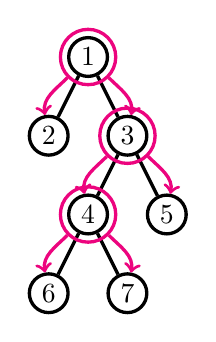
\begin{tikzpicture}[xscale = 1, yscale = 1, very thick]
                \tikzstyle{vertex}=[circle, draw = black,fill=white,minimum size=14pt,inner sep=0pt]
                
                \foreach \name/\x/\y in {1/0/3, 2/-0.5/2, 3/0.5/2, 4/0/1, 5/1/1, 6/-0.5/0, 7/0.5/0}
                \node[vertex] (G-\name) at (\x,\y) {\name};
                
                \foreach \from/\to in {1/2, 1/3, 3/4, 3/5, 4/6, 4/7}
                \draw (G-\from) -- (G-\to);
    
        \node<2->[circle, draw = RubineRed, very thick, minimum size = 20pt, fill = none](emph1) at (0,3){};
        
        \draw<3->[RubineRed, very thick, ->] (emph1) to [out = 225, in=100] (G-2);
        
        \draw<4->[RubineRed, very thick, ->] (emph1) to [out = 315, in=80] (G-3);
        
        \node<5->[circle, draw = RubineRed, very thick, minimum size = 20pt, fill = none](emph3) at (0.5,2){};
    
         \draw<6->[RubineRed, very thick, ->] (emph3) to [out = 225, in=100] (G-4);
    
        \draw<7->[RubineRed, very thick, ->] (emph3) to [out = 315, in=80] (G-5);
    
        \node<8->[circle, draw = RubineRed, very thick, minimum size = 20pt, fill = none](emph4) at (0,1){};
    
      \draw<9->[RubineRed, very thick, ->] (emph4) to [out = 225, in=100] (G-6);
    
        \draw<10->[RubineRed, very thick, ->] (emph4) to [out = 315, in=80] (G-7);
       
            \end{tikzpicture}
            \end{minipage}
            \hfill
            \begin{minipage}[b]{0.69 \textwidth}
                Stochastic construction, root = 1
                \medskip\\
                \onslide<2->{$N_1 = L_1,\phantom{+\;\alpha_{(v,2)}\circ N_1}\quad L_1\sim$ Poisson$(\lambda)$}\\
                \onslide<3->{$N_2 = \alpha_{(1,2)}\circ N_1 + L_2,\quad L_2\sim$ Poisson$(\lambda(1-\alpha_{(1,2)}))$}\\
                \onslide<4->{$N_3 = \alpha_{(1,3)}\circ N_1 + L_3,\quad L_3\sim$ Poisson$(\lambda(1-\alpha_{(1,3)}))$}\\
                \onslide<6->{$N_4 = \alpha_{(3,4)}\circ N_3 + L_4,\quad L_4\sim$ Poisson$(\lambda(1-\alpha_{(3,4)}))$}\\
                \onslide<7->{$N_5 = \alpha_{(3,5)}\circ N_3 + L_5,\quad L_5\sim$ Poisson$(\lambda(1-\alpha_{(3,5)}))$}\\
                \onslide<9->{$N_6 = \alpha_{(4,6)}\circ N_4 + L_6,\quad L_6\sim$ Poisson$(\lambda(1-\alpha_{(4,6)}))$}\\
                 \onslide<10->{$N_7 = \alpha_{(4,7)}\circ N_4 + L_7,\quad L_7\sim$ Poisson$(\lambda(1-\alpha_{(4,7)}))$}
            \end{minipage}
        \end{figure}
     where "$\circ$" is the binomial thinning operator: $(\alpha\circ N) \sim$ Binomial$(N,\alpha)$
            %\caption{$\mathcal{T}$, with $\mathcal{V} = \{1,\dots,5\}$     and $\mathcal{E} = \{(1,2), (1,3), (3,4), (3,5)\}$}
            %\label{fig:GrapheChaineMarkov}
        \end{example}
    \end{frame}

\begin{frame}
    \frametitle{Individual Risk Models}
    Lorem ipsum dolor sit amet:
    \begin{itemize}
    \item Here is a basic alert: \al{important text}
    \item Here is a basic alert on the second click: \al[2]{important text}
    \item Here is a positive alert on the third click: \alg[3]{important text}
    \item Here are various alerts to flag the sign of numbers:
    \begin{itemize}
    \item Positive number: \alg{+5}
    \item Negative number: \alr{-10}
    \item Zero number: \alb{0.0}
    \end{itemize}
    \item Here are the same alerts on the second and third clicks:
    \begin{itemize}
    \item Positive number: \alg[2-3]{+5}
    \item Negative number: \alr[2]{-10}
    \item Zero number: \alb[3]{0.0}
    \end{itemize}
    \end{itemize}
    \end{frame}

\appendix

\begin{frame}[allowframebreaks]{References}
\bibliography{references}
\bibliographystyle{apalike}
\end{frame}

% \lastslide

% \begin{frame}[label=backupSlide]
% \frametitle{First backup slide}
% \begin{itemize}
% \item Lorem ipsum dolor sit amet, consectetur adipisicing elit, sed do eiusmod
% tempor incididunt ut labore et dolore magna aliqua.
% \item  Ut enim ad minim veniam, quis nostrud exercitation ullamco laboris nisi ut aliquip ex ea commodo consequat. 
% \item Duis aute irure dolor in reprehenderit in voluptate velit esse
% cillum dolore eu fugiat nulla pariatur. 
% \end{itemize}
% \hyperlink{firstSlide}{\beamergotobutton{Return to main slide}}
% \end{frame}

% \begin{frame}[label=anotherBackupSlide]
% \frametitle{Another backup slide}
% \begin{enumerate}
% \item  Ut enim ad minim veniam, quis nostrud exercitation ullamco laboris nisi ut aliquip ex ea commodo consequat. 
% \item Lorem ipsum dolor sit amet, consectetur adipisicing elit, sed do eiusmod
% tempor incididunt ut labore et dolore magna aliqua.
% \begin{enumerate}
% \item Duis aute irure dolor in reprehenderit in voluptate velit esse
% \item Cillum dolore eu fugiat nulla pariatur
% \end{enumerate}
% \item Lorem ipsum dolor sit amet, consectetur adipisicing elit, sed do eiusmod
% tempor incididunt ut labore et dolore magna aliqua.
% \end{enumerate}
% \hyperlink{firstSlide}{\beamergotobutton{Return to main slide}}
% \end{frame}

\end{document}